\documentclass [tikz] {standalone}
\begin{document}    

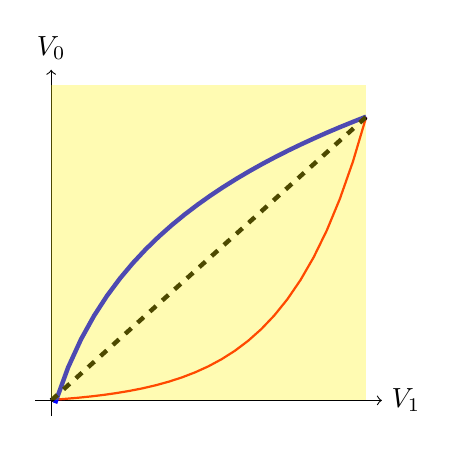
\begin{tikzpicture}[domain=0.55:4.5]
    \draw[->] (-0.2,0) -- (4.2,0) node[right] {$V_1$};
    \draw[->] (0,-0.2) -- (0,4.2) node[above] {$V_0$};
    \draw[color=red, thick,domain=0:4] plot (\x,{0.067*exp(\x) - 0.06});
    \draw[color=blue, ultra thick] plot (\x - 0.5,{1.2*log2(\x) + 1});
    \draw[color=black, ultra thick, dashed, domain=0:4] plot (\x,{0.9*(\x)});
    \fill[yellow, fill opacity = 0.3] (0,0)   rectangle (4,4);
      
\end{tikzpicture}

\end{document}